\subsection*{Neutrinos de Majorana}
Una de las preguntas más importantes que se plantea la física de partículas moderna es la de si el neutrino es su propia antipartícula, tal como fue postulado por el físico italiano Ettore Majorana, alrededor de 1930. La importancia de esta cuestión radica en la necesidad, por parte de las teorías de leptogénesis, de introducir neutrinos de Majorana como un ingrediente esencial para generar la asimetría cósmica entre materia y antimateria. La presencia de neutrinos de Majorana pesados también permitiría explicar el hecho de que las masas de los neutrinos ligeros sea mucho más pequeña que la de los correspondientes leptones. 

La desintegración doble beta (\bb) es un proceso débil de segundo orden en el que un núcleo con número atómico Z y masa atómica A se transforma en su isóbaro con número atómico 
Z+2:

\begin{equation}
(Z,A) \rightarrow (Z+2,A) + 2 e^- + 2 \bar{\nu}_e 
\end{equation}
%                                     
Los procesos \bb\ han sido observados en numerosos isótopos, midiéndose vidas medias en el rango de $10^{18} - 10^{21}$ años. Se trata del proceso de desintegración radioactiva más lento que se conoce. Sólo se observa en 35 isótopos naturales, en los que la desintegración beta convencional al núcleo (Z+1) está suprimida o prohibida energéticamente. 

Por otra parte la desintegración doble beta sin neutrinos (\bbonu):
                                     
\begin{equation}
(Z,A) \rightarrow (Z+2,A) + 2 e^- 
\end{equation}
 %                                    
sólo puede darse si los neutrinos son partículas de Majorana. El mecanismo más sencillo para producir esta desintegración implica el intercambio de neutrinos ligeros y viene caracterizado por una vida media \Tonu\ cuya inversa es proporcional al cuadrado de la llamada masa efectiva de Majorana, \mbb: 
                                    
\begin{equation}
(\Tonu)^{-1} =\Gonu \Monu^2 \mbb^2 ,
\label{eq.t0nu}
\end{equation}
%  
donde el término \Gonu\ es un factor de espacio de fases y el término \Monu\ un elemento de matriz nuclear. La masa  de Majorana, \mbb\ , es una superposición de los tres autoestados de masa de los neutrinos, ${\rm m_i ~(i=1,3)} $: 
                                    
\begin{equation}
\mbb =|m_1 |U_{e1}|^2 + m_2 |U_{e2}|^2 e^{i\alpha}+ m_3 |U_{e3}|^2 e^{i\beta}| ,
\label{eq.mbb}
\end{equation}
%
donde los factores $U_{ei}$~ son elementos de la matriz de mezcla leptónica y $\alpha,\beta$ son las llamadas fases de Majorana. Así pues, el periodo de la desintegración \bbonu\ aumenta a medida que la masa de Majorana se hace más y más ligera. Los límites actuales en el periodo \Tonu\  (del orden de 10$^{25}$~ años) pueden traducirse en límites en la masa de \mbb\ (del orden de 130-300 meV). La considerable incertidumbre en dichos límites se debe a las dificultades teóricas para calcular el elemento de matriz nuclear \Monu.  

Desde el punto de vista experimental, la desintegración \bbonu\ ofrece una señal característica. En efecto, la ausencia de neutrinos se traduce en que la suma de las energías cinéticas de los dos electrones emitidos en el proceso es siempre la misma, e igual a \Qbb: 
                                    
\begin{equation}
\Qbb =M(A,Z) - M(A, Z+2)
\label{eq.mbb}
\end{equation}
%
Por tanto, para un experimento de \bbonu\ es importante medir con buena resolución  la energía de los dos electrones. En el límite de un detector de resolución perfecta, bastaría con observar una desintegración tal que la suma de las energías de los dos electrones fuera idéntica a \Qbb\  para establecer que se trata de una desintegración \bbonu. En la práctica, incluso los detectores con mejor resolución energética (basados en cristales semiconductores de germanio o bolómetros de telurio) miden una distribución de energía con una cierta anchura a media altura (FWHM) del orden de unos pocos keV. Por otra parte, las vidas medias del proceso \bbonu\ son muy largas. Teniendo en cuenta que los ruidos de fondo a este proceso están relacionados con las cadenas naturales del uranio y el torio, con vidas medias características de $10^{10}$~ años, nos encontramos con que los experimentos \bbonu\ deben reducir los potenciales ruidos de fondo en más de 15 órdenes de magnitud. 

\subsection*{El experimento NEXT}

Uno de los mejores isótopos para buscar procesos \bbonu\ es el \XE. El xenón es un gas noble, que permite construir aparatos que sean simultáneamente blanco y  detector, aprovechando las propiedades de centelleo e ionización del gas. En concreto, el experimento NEXT propone la construcción de cámaras de proyección temporal (TPCs) utilizando xenón a alta presión (HPXe) y amplificando la señal de ionización mediante electroluminescencia (EL). El gas xenón está enriquecido al 90\% en \XE. 


\begin{figure}
\centering
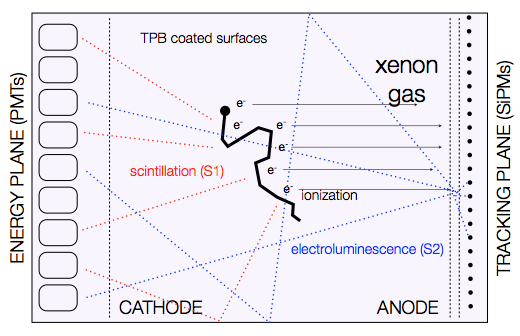
\includegraphics[width=0.8\textwidth]{img/EL.png}
\caption{\small Principio de operación del detector NEXT. 
} \label{fig.EL}
\end{figure}
                                    
El principio de operación de NEXT se ilustra en la Figura \ref{fig.EL}. Cuando se produce un suceso ionizante en el xenón (sea este una desintegración \bb\ o un suceso de ruido de fondo, por ejemplo la interacción Compton o fotoeléctrica de un fotón de alta energía) la respuesta del gas es la emisión de luz de centelleo ultravioleta (UV) con una longitud de onda cuyo pico se sitúa en 172 nm. Esta luz de centelleo es copiosa (del orden de 60,000 fotones por MeV de energía depositada) y, como se verá, constituye la base de funcionamiento de PETALO, descrito posteriormente en esta memoria. En el detector NEXT el centelleo primario permite medir el tiempo inicial (\tto) de la interacción.

Los electrones de ionización producidos por el paso de la radiación son arrastrados en el detector NEXT hacia el ánodo, merced a un campo eléctrico de unos 300 V/cm. Antes de llegar al ánodo, los electrones atraviesan una rejilla situada a un potencial de unos 15,000 voltios con respecto al ánodo. Como consecuencia, los electrones se aceleran, emitiendo del orden de 1,000 fotones ultravioleta durante el tiempo que necesitan para cruzar la llamada región de electroluminescencia. Estos fotones se emiten isotrópicamente. Los fotones que se propagan hacia el ánodo son registrados por un plano de detectores de estados sólido llamados fotomultiplicadores de silicio (SiPMs) situado detrás de este. Los fotones que se propagan en otras direcciones llegan hasta un plano de fotomultiplicadores convencionales (PMTs) situados tras el cátodo. El plano de SiPMs se llama plano de trazado y, permite reconstruir la trayectoria de los electrones primarios. El plano de PMTs se llama plano de energía y permite reconstruir la energía del evento. 

La tecnología de NEXT conjunta varias ventajas importantes para la realización óptima de un experimento \bbonu:
                                    
                                    %%%%%
\begin{figure}
\centering
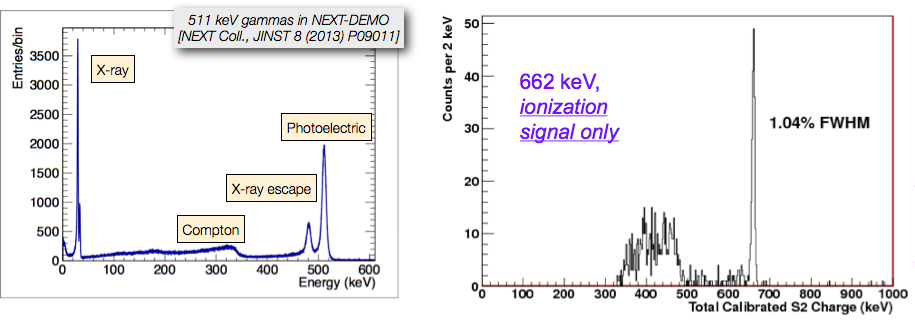
\includegraphics[width=0.7\textwidth]{img/EResolution.png}
\caption{\small Izquierda: Espectro de energía medido para electrones de 511 keV en el detector NEXT-DEMO. Derecha: El espectro cerca del pico fotoeléctrico a 662 keV. La resolución at 662 keV es 1\% FWHM, lo que extrapola a 0.5\% FWHM en \Qbb.}
\label{fig.ERES}. 
\end{figure}
%%%%

%%%%%
\begin{figure}
\centering
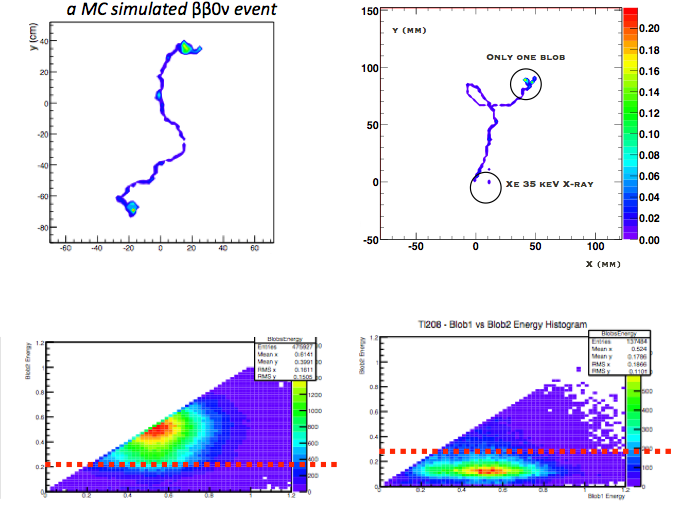
\includegraphics[width=0.7\textwidth]{img/Topo2.png}
\caption{\small NEXT es uno de los pocos experimentos de búsqueda \bbonu\ que puede proporcionar una señal topológica. El panel superior izquierdo muestra la reconstrucción de un suceso de señal (generado por Monte Carlo), que consiste en dos electrones producidos en un vértice común. El panel superior derecho muestra un evento de ruido de fondo, que consiste en un electrón emitido por los isótopos  \BI\ o \TL. En el caso de la señal, aparecen dos bolas de energía depositadas en los extremos de la traza, mientras que el ruido de fondo muestra sólo una bola. En los paneles inferiores se representa la energía de las dos bolas que se encuentran en los extremos de la traza. En el caso de la señal (panel inferior izquierdo) la energía de ambas bolas es alta y aproximadamente igual. En el caso del ruido de fondo (panel inferior derecho) la energía de una de las bolas es muy pequeña. Un simple corte, requiriendo que la energía de ambas bolas sea superior a 0.2 MeV, separa eficientemente la señal del ruido.}\label{fig.ETRK2}
\end{figure}
%%%%%

\begin{enumerate}
\item {\bf Excelente resolución en energía} (Figura \ref{fig.ERES}) medida por la colaboración NEXT usando los prototipos NEXT-DEMO y NEXT-DBDM, desarrollados en la fase de I+D+i del experimento . Se obtiene una resolución de 0.5 \% FWHM en la zona de interés cercana a \Qbb. La resolución en energía de NEXT es un factor 8 superior a la del experimento EXO, basado en una cámara de xenón líquido y superior en un factor 20 a la del experimento KamLAND-Zen, donde el gas se disuelve en centellador líquido. 
\item {\bf Caracterización de la señal mediante una señal topológica} (Figura \ref{fig.ETRK2}). NEXT puede reconstruir la señal de los dos electrones emitidos en una desintegración \bb\, distinguiéndolos de la señal que proporcionan los ruidos de fondo, constituidos mayoritariamente por un solo electrón.
\item {\bf Alta radiopureza en los materiales que constituyen el detector}, minimizando contaminaciones radioactivas (trazas de las cadenas de uranio y torio) que puedan enmascarar la señal \bbonu.
\item {\bf La tecnología puede escalarse fácilmente a altas masas}. Al tratarse de detector continuo (el xenón es a la vez blanco y detector), cada vez que se doblan las dimensiones longitudinales del aparato se multiplica su masa por un factor de, aproximadamente $2^3$, mientras que la superficie escala como $2^2$. Dado que la señal es proporcional a la masa del blanco y los ruidos de fondo son aproximadamente proporcionales a las superficies del detector (donde se depositan las trazas radioactivas que los originan), cada vez que se doblan las dimensiones del detector se mejora la señal sobre el ruido en un factor $2^3/2^2 = 2$. 
\end{enumerate}

La economía de escala que presenta la tecnología  ha permitido la construcción de una serie de detectores para establecer progresivamente la validez de la tecnología y entender el impacto de los ruidos de fondo. El primero de estos detectores, NEXT-DEMO, permitió desarrollar los aspectos tecnológicos, muy novedosos, de las HPXe-EL y demostró, con una masa de 1 kg, excelente resolución en energía, así como una robusta señal topológica. En la actualidad, el detector NEW, con una masa de 10 kg, está comenzando a operar en el LSC y medirá con precisión los ruidos de fondo ambientales esperados en el experimento. El detector NEXT-100, con una masa de 100 kg, empezará a operar en el LSC en 2018. 


\begin{figure}
\centering
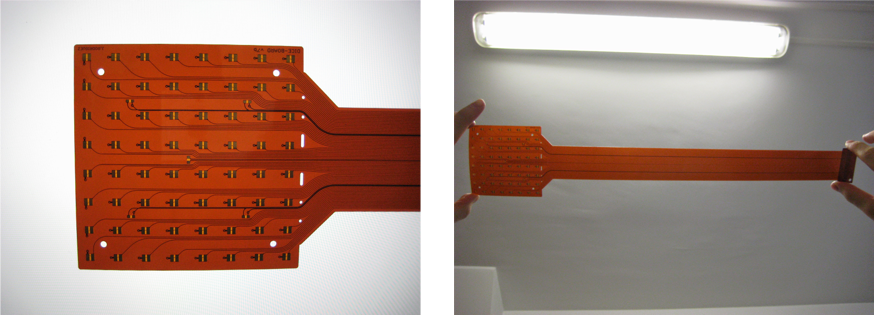
\includegraphics[width=0.8\textwidth]{img/KDB.png}
\caption{\small Los Kapton Dice Boards (KDB) de NEXT.} \label{fig.KDB}
\end{figure} 


Uno de los elementos más novedosos de NEXT es su plano de trazado que permite la reconstrucción de las trayectorias de los electrones en el gas. El plano de trazado está formado por matrices de SiPMs, organizadas en circuitos de kapton, llamados KDBs (de las siglas en inglés de Kapton Dice Boards). La Figura \ref{fig.KDB} muestra uno de estos KDBs, que suponen un diseño original de NEXT. El detector NEW cuenta con unos 25 KDBs, cada uno de los cuales tiene 64 SiPMs (1,600 canales en total). El detector NEXT-100 cuenta con 110 KDBs  (7040 canales).  

NEXT-100 podría descubrir la existencia de procesos \bbonu\ si su periodo es de hasta $10^{26}$~años. En caso contrario, la siguiente fase, denominada NEXT2N (next-to-next) contemplaría la construcción de un detector con una masa de centenares de kilos capaz de explorar periodos \Tonu\ del orden de $10^{27}$~años. {\bf En consecuencia, un experimento construido y en operación en España y liderado desde la Comunidad Valenciana, podría situarse al frente del campo de la física \bbonu\ en los próximos años}.
 
 
\begin{figure}
\centering
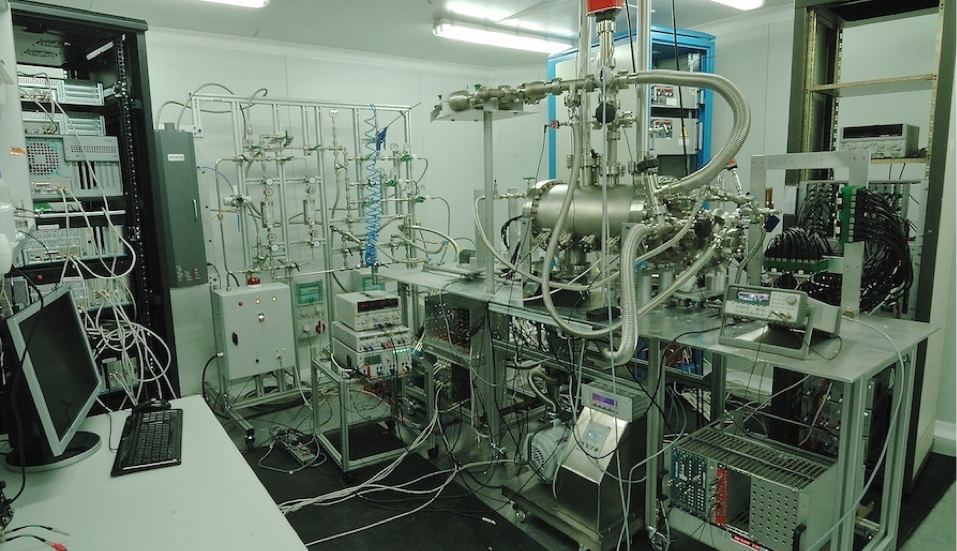
\includegraphics[width=0.6\textwidth]{img/DemoSetup.png}
\caption{\small El detector NEXT-DEMO en el laboratorio del IFIC (Valencia).} \label{fig.DEMO}
\end{figure}

%%%%%%%%%%
\begin{figure}
\centering
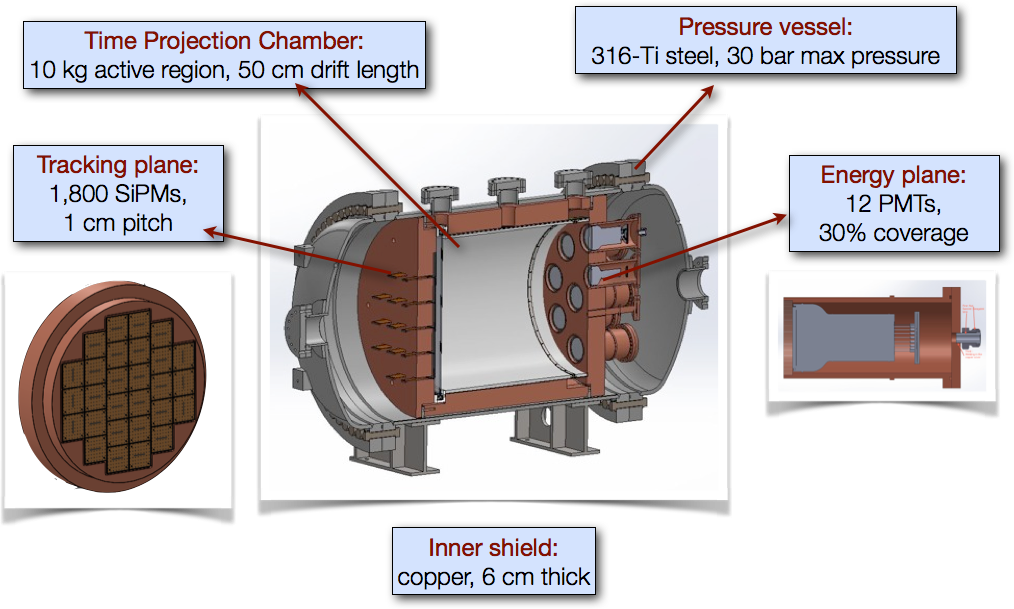
\includegraphics[width=0.6\textwidth]{img/NEW.png}
\caption{\small NEW, la primera fase del experimento NEXT en Canfranc.} \label{fig:NEW}
\end{figure} 

%%%%%%%%%%
\begin{figure}
\centering

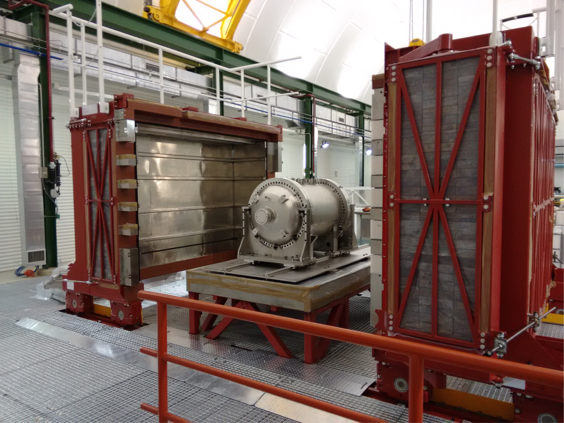
\includegraphics[width=0.6\textwidth]{img/NewCastle.png}
\caption{\small El detector NEW, instalado en el Castillo de Plomo que blinda el experimento de la radiación exterior.} \label{fig.NewCastle}
\end{figure} 

\begin{figure}
\centering
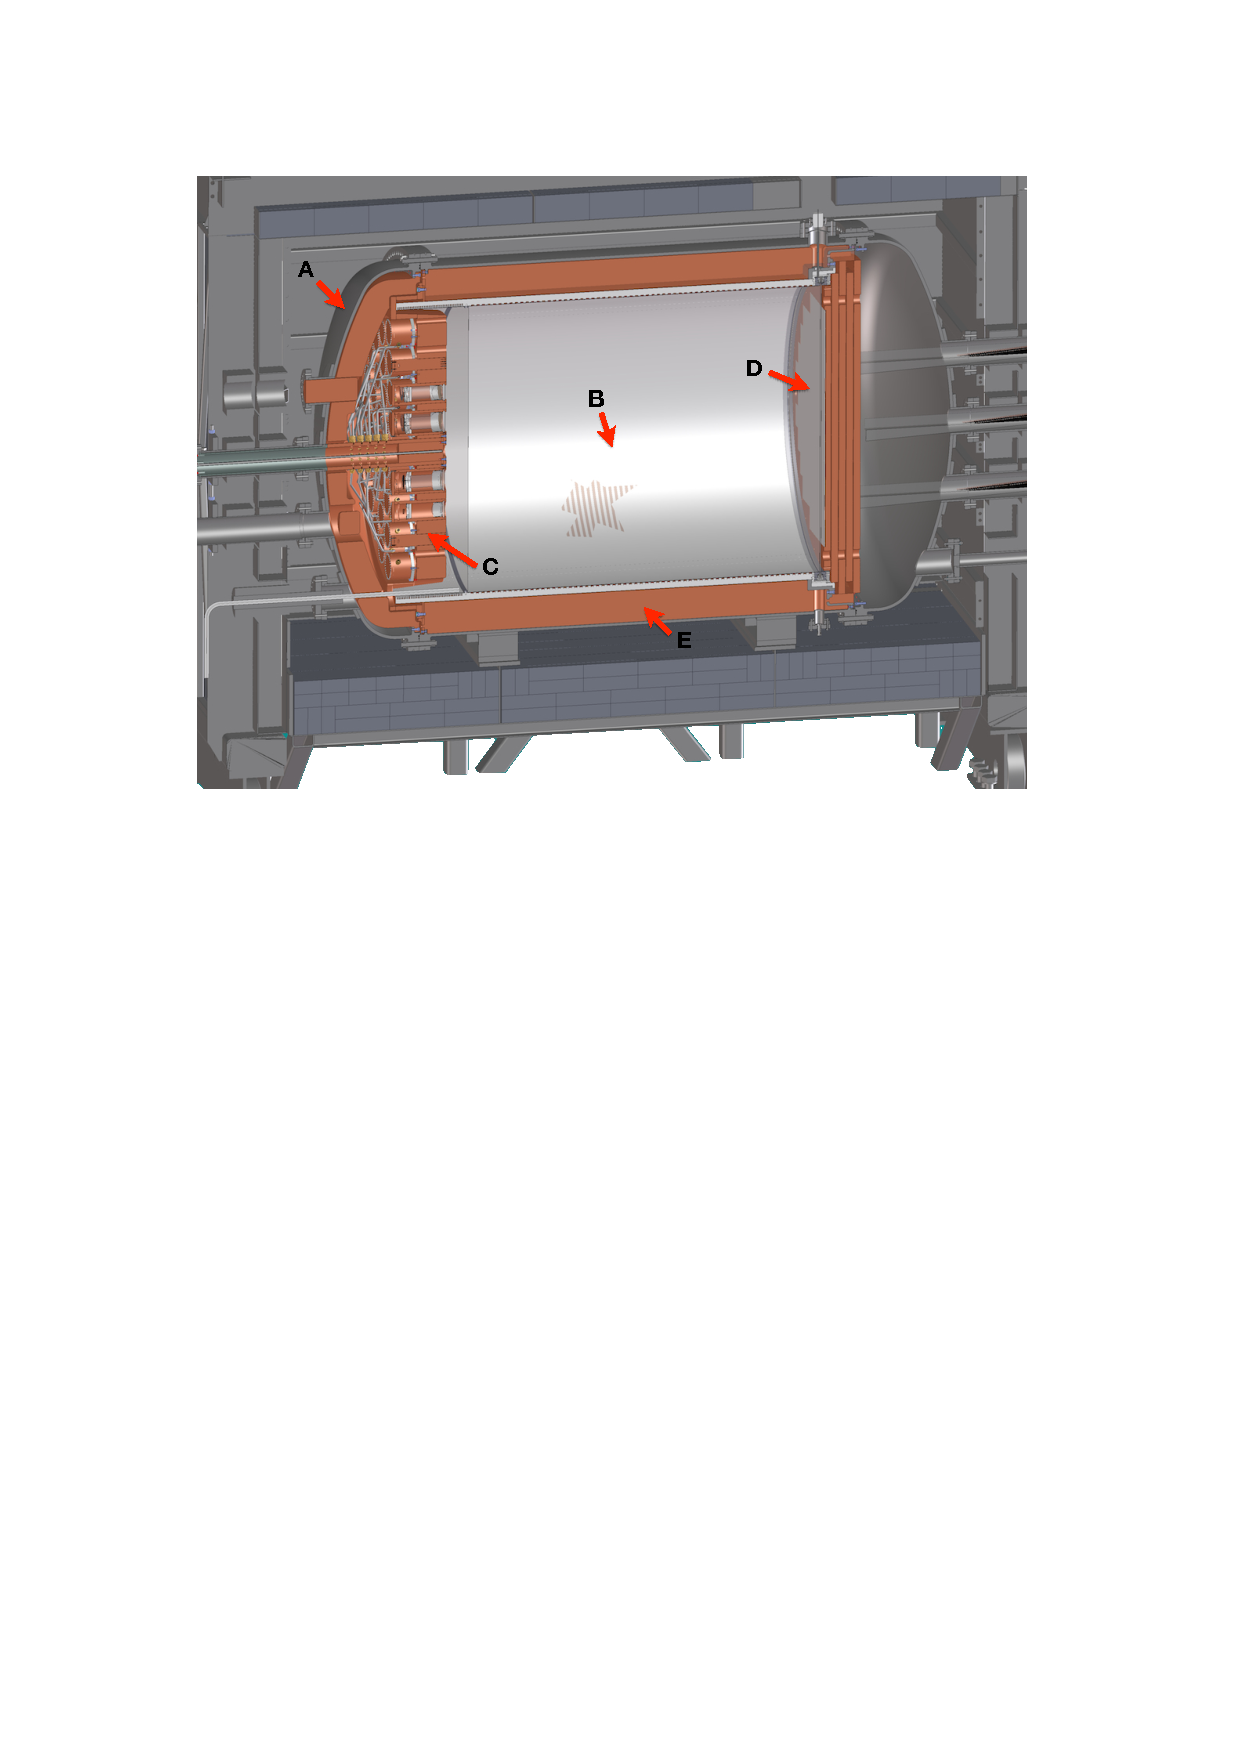
\includegraphics[width=0.6\textwidth]{img/NEXT100.pdf}
\caption{\small Sección transversal del detector NEXT-100, localizado en el interior del blindaje de plomo. Una vasija de presión hecha de acero-titanio (A) alberga la jaula eléctrica (B) y los dos planos de sensores (plano de trazado, C, plano de energía, D), localizados en los extremos de la cámara. El volumen activo está aislado de la radiación exterior por 12 cm de cobre (E).
} \label{fig.NEXT100}
\end{figure}

El experimento NEXT se ha desarrollado en varias fases. 
 \begin{enumerate}
\item Primera fase, correspondiente a I+D+i, que abarcó desde 2008 hasta 2014. Los hitos fundamentales de esta fase fueron la construcción y operación del detector NEXT-DEMO (Figura \ref{fig.DEMO}) que ha demostrado el gran potencial de la novedosa tecnología HPXe-EL en la que se basa NEXT. 
\item Segunda fase, correspondiente a la operación en el LSC del detector NEW (Figura \ref{fig:NEW}), que está siendo puesto a punto en el LSC durante 2015 (Figura \ref{fig.NewCastle}) y empezará a tomar datos en 2016. NEW operará por un periodo de 2 años (2016 y 2017) y su objetivo principal es medir los ruidos de fondo radioactivos, así como establecer y probar todas las infraestructuras necesarias (sistema de gas, sistemas automáticos de control y seguridad, sistema de blindaje, sistema de supresión de radón) para la operación de NEXT-100.
\item Tercera fase, correspondiente a  la operación en el LSC del detector NEXT-100  (Figura \ref{fig.NEXT100}). Esta fase empezará en 2018 y podría extenderse durante 3 años.
 El objetivo de NEXT-100 es alcanzar un periodo 
$\Tonu \sim 10^{26}$, explorando por tanto una región aún no estudiada, donde un descubrimiento sería posible.  Otros experimentos (GERDA-II, CUORE, KamLAND-ZEN, EXO y SNO+) intentarán también encontrar este proceso durante los próximos años, utilizando diversas técnicas e isótopos, por lo que es posible que se produzca un descubrimiento, del que NEXT podría ser parte, combinando varias técnicas e isótopos. 
\item Cuarta fase (detector NEXT2N) que podría empezar a partir de 2021, con la construcción de un detector en el rango de 300--500 kg, en el que además se reduciría el ruido de fondo específico de NEXT-100, mediante una serie de mejoras que se desarrollarán en los próximos años y que incluyen: a) sustituir los PMTs del plano de energía por SiPMs de gran área; b) introducir electrónica de digitalización en el interior de la cámara, mediante ASIC especializados; c) reducir la difusión en el xenón, mediante la adición de mezclas apropiadas (e.g, una mezcla con 0.1\% de CH$_4$~ está siendo estudiada en la actualidad); En general todas etas mejoras van en la dirección de reducir la radioactividad de los componentes de NEXT y de mejorar tanto su resolución en energía como la señal topológica. 
\end{enumerate}


\subsection*{Objetivos: NEXT}

El primer objetivo de este proyecto es contribuir de manera decisiva al desarrollo del experimento NEXT. Los objetivos específicos son los siguientes:

\subsubsection*{Operación de los detectores NEW y NEXT-100 en el LSC}

Tanto NEW como NEXT operarán de manera rutinaria durante las 24 horas del día, por un periodo de 10 meses al año (no se opera durante el mes de Agosto, ya que el LSC cierra por descanso anual y las operaciones de mantenimiento requieren unas cuatro semanas al año). Durante todo el periodo de operación es necesaria la presencia de miembros del equipo NEXT en el laboratorio. La regulación del LSC requiere que haya siempre dos personas en las instalaciones subterráneas, lo cual define el tamaño mínimo del equipo. Durante las épocas de instalación o mantenimiento, el número de físicos e ingenieros de NEXT suele ser de 6-8 personas.

La forma de operación habitual en una colaboración internacional como NEXT es repartir turnos de trabajo entre los científicos e ingenieros que integran la colaboración. No obstante, el grupo del IFIC es responsable de la coordinación de operaciones y el grupo de la UPV de la dirección organizativa (project management). La operación de los detectores requiere la presencia en el LSC del coordinador de operaciones (IFIC) y, con mucha frecuencia del Project Manager (UPV) y del coordinador técnico (IFIC). 

\subsubsection*{Análisis de datos de los detectores NEW y NEXT-100} 

Durante 2016 y 2017 el análisis de los datos del detector NEW permitirá una detallada caracterización de los parámetros operativos de NEXT (resolución en energía, señal topológica) así como de los principales ruidos de fondo. Durante 2018 y 2019 el análisis de los datos de NEXT-100 se centrará en la búsqueda de procesos \bbonu. El grupo del IFIC incluye el coordinador de software y el coordinador de análisis, que lideran estas actividades. 

Entre los trabajos a realizar en la fase NEW se cuentan: i) la calibración de los detectores con fuentes radiactivas (\ensuremath{^{83}}Kr, \NA, \CS, etc.); ii) la medida de la resolución en energía y su dependencia con la energía de operación; c) el estudio detallado de la señal topológica; d) el estudio detallado del impacto de los ruidos de fondo, en particular de las emanaciones internas de radón. Durante la fase NEXT-100 se procederá a la búsqueda de sucesos \bb\ y de sucesos \bbonu, utilizando varios análisis independientes, tanto en técnicas de filtrado (análisis convencional en el que la señal se selecciona estableciendo cortes de selección en diversas variables frente a análisis en los que se aplican técnicas de multi-variaciones o redes neuronales) como en los equipos que los llevan a cabo. El grupo del IFIC tendrá un papel de líder en la mayoría de estas actividades. 
 
\subsubsection*{Mejora de la electrónica de NEXT}

Tanto NEW como NEXT-100 operan con electrónica COTS
(de las siglas en inglés {\em commercial of the shelf}, esto es electrónica comercial disponible en el mercado) que ha sido desarrollada por el grupo de la UPV. Pese a su alta fiabilidad y buen rendimiento, la solución actual presenta algunos problemas que podrían mejorarse en el detector NEXT-100. En particular, las señales de los SiPMs y los PMTs son digitalizadas fuera de la cámara y por tanto es necesario extraerlas mediante cables de considerable longitud (del orden de 10 metros), hasta los convertidores analógico-digitales (ADCs) situados en el exterior del blindaje del detector. En el caso de NEW, se precisa, por tanto, extraer 25 cables planos (uno por KDB), a través de pasamuros diseñados para resistir la presión de operación (15 atmósferas) y para minimizar las fugas de xenón a través de ellos hasta niveles inferiores a 1 gramo por año. En el caso de NEXT-100 se precisará extraer más de 100 cables. 

El uso de electrónica COTS resulta mucho más complejo aún para la cuarta fase de NEXT, ya que se prevé que el detector NEXT2N sea un detector simétrico (SiPMs tanto en el plano de energía como en el plano de trazado) con masa en el rango de 300 a 500 kg. El número  de cables (y por tanto de pasamuros), si se opta por la misma solución adoptada por NEW y NEXT-100, sería del orden de 500. 

Una alternativa muy interesante para NEXT2N sería digitalizar la señal en el interior de la cámara, mediante ASICs especializados y extraer la señal digital, serializada, mediante fibra óptica. Esta solución, propuesta recientemente por el grupo de la UPV, minimizaría el número de pasamuros y permitiría reducir costes.

Por otra parte, como se comenta más tarde, existe la posibilidad de utilizar el mismo ASIC que se propone para el aparato PETALO como ASIC para el plano de trazado de NEXT. Además, el ASIC que se propone es un producto comercial ya existente y con un precio muy competitivo. Demostrar la viabilidad de esta solución es un importantísimo objetivo par el futuro del experimento. 


\subsection*{Desarrollo del proyecto}
Las actividades a realizar en el proyecto NEXT durante los próximos cuatro años son:
\begin{enumerate}
\item {\bf 2016}: operación del detector NEW. Calibración, estabilidad, control de riesgos (slow control), puesta a punto de la electrónica, medida de la resolución en energía y señal topológica.
\item {\bf 2017}: Medida de ruidos de fondo con el detector NEW y caracterización del modelo de ruido de fondo para NEXT. 
\item {\bf 2018}: Construcción y puesta a punto del detector NEXT-100. 
\item {\bf 2019}: Operación del detector NEXT-100. Búsqueda de señales \bbonu.  Sustitución de la electrónica del plano de trazado de NEW con electrónica ASIC para demostrar la viabilidad de esta solución para NEXT2N. 


\end{enumerate}

\subsection*{Financiación del proyecto}

La fase de I+D+i del experimento NEXT fue financiada por un proyecto CONSOLIDER-INGENIO, llamado CUP. Durante esta fase se construyó y operó el detector NEXT-DEMO. La construcción  detector NEW, así como del detector NEXT-100 cuentan con la financiación de un AdG/ERC y un proyecto coordinado de la convocatoria RETOS 2014. La financiación existente, sin embargo, no cubre todas las necesidades de personal y de operación del experimento. En este proyecto se solicita financiación para contribuir a la operación de NEW, así como para un contrato de ingeniero compartido con el proyecto PETALO, como se detalla más adelante. También se solicita financiación para demostrar la viabilidad de una electrónica digital en el interior de la cámara, para lo cual se propone sustituir la electrónica del plano de trazado de NEW con electrónica ASIC. 

